% Options for packages loaded elsewhere
\PassOptionsToPackage{unicode}{hyperref}
\PassOptionsToPackage{hyphens}{url}
%
\documentclass[
]{article}
\usepackage{amsmath,amssymb}
\usepackage{iftex}
\ifPDFTeX
  \usepackage[T1]{fontenc}
  \usepackage[utf8]{inputenc}
  \usepackage{textcomp} % provide euro and other symbols
\else % if luatex or xetex
  \usepackage{unicode-math} % this also loads fontspec
  \defaultfontfeatures{Scale=MatchLowercase}
  \defaultfontfeatures[\rmfamily]{Ligatures=TeX,Scale=1}
\fi
\usepackage{lmodern}
\ifPDFTeX\else
  % xetex/luatex font selection
\fi
% Use upquote if available, for straight quotes in verbatim environments
\IfFileExists{upquote.sty}{\usepackage{upquote}}{}
\IfFileExists{microtype.sty}{% use microtype if available
  \usepackage[]{microtype}
  \UseMicrotypeSet[protrusion]{basicmath} % disable protrusion for tt fonts
}{}
\makeatletter
\@ifundefined{KOMAClassName}{% if non-KOMA class
  \IfFileExists{parskip.sty}{%
    \usepackage{parskip}
  }{% else
    \setlength{\parindent}{0pt}
    \setlength{\parskip}{6pt plus 2pt minus 1pt}}
}{% if KOMA class
  \KOMAoptions{parskip=half}}
\makeatother
\usepackage{xcolor}
\usepackage[margin=1in]{geometry}
\usepackage{graphicx}
\makeatletter
\def\maxwidth{\ifdim\Gin@nat@width>\linewidth\linewidth\else\Gin@nat@width\fi}
\def\maxheight{\ifdim\Gin@nat@height>\textheight\textheight\else\Gin@nat@height\fi}
\makeatother
% Scale images if necessary, so that they will not overflow the page
% margins by default, and it is still possible to overwrite the defaults
% using explicit options in \includegraphics[width, height, ...]{}
\setkeys{Gin}{width=\maxwidth,height=\maxheight,keepaspectratio}
% Set default figure placement to htbp
\makeatletter
\def\fps@figure{htbp}
\makeatother
\setlength{\emergencystretch}{3em} % prevent overfull lines
\providecommand{\tightlist}{%
  \setlength{\itemsep}{0pt}\setlength{\parskip}{0pt}}
\setcounter{secnumdepth}{-\maxdimen} % remove section numbering
\usepackage{booktabs}
\usepackage{longtable}
\usepackage{array}
\usepackage{multirow}
\usepackage{wrapfig}
\usepackage{float}
\usepackage{colortbl}
\usepackage{pdflscape}
\usepackage{tabu}
\usepackage{threeparttable}
\usepackage{threeparttablex}
\usepackage[normalem]{ulem}
\usepackage{makecell}
\usepackage{xcolor}
\ifLuaTeX
  \usepackage{selnolig}  % disable illegal ligatures
\fi
\usepackage{bookmark}
\IfFileExists{xurl.sty}{\usepackage{xurl}}{} % add URL line breaks if available
\urlstyle{same}
\hypersetup{
  pdftitle={Preguntas\_exploratorias2},
  pdfauthor={Irving, Chuy},
  hidelinks,
  pdfcreator={LaTeX via pandoc}}

\title{Preguntas\_exploratorias2}
\author{Irving, Chuy}
\date{2025-01-31}

\begin{document}
\maketitle

\subsubsection{1 ¿Cuáles son las 10 películas que contaron con más
presupuesto?}\label{cuuxe1les-son-las-10-peluxedculas-que-contaron-con-muxe1s-presupuesto}

\begin{verbatim}
##                                            title    budget
## 717  Pirates of the Caribbean: On Stranger Tides 380000000
## 4711                     Avengers: Age of Ultron 365000000
## 5953                           Avengers: Endgame 356000000
## 164     Pirates of the Caribbean: At World's End 300000000
## 4954                              Justice League 300000000
## 5954                      Avengers: Infinity War 300000000
## 608                             Superman Returns 270000000
## 3792                                     Tangled 260000000
## 7135                               The Lion King 260000000
## 281                                 Spider-Man 3 258000000
\end{verbatim}

\subsubsection{3 ¿Cuál es la película que más votos
tuvo?}\label{cuuxe1l-es-la-peluxedcula-que-muxe1s-votos-tuvo}

\begin{verbatim}
##          title voteCount
## 3512 Inception     30788
\end{verbatim}

\subsubsection{5 ¿Cuántas películas se hicieron en cada año? ¿En qué año
se hicieron más películas? Usar un gráfico de
barras}\label{cuuxe1ntas-peluxedculas-se-hicieron-en-cada-auxf1o-en-quuxe9-auxf1o-se-hicieron-muxe1s-peluxedculas-usar-un-gruxe1fico-de-barras}

\begin{verbatim}
## # A tibble: 99 x 2
##     Anio Cantidad
##    <dbl>    <int>
##  1  2021      816
##  2  2018      629
##  3  2017      618
##  4  2019      612
##  5  2016      557
##  6  2020      533
##  7  2015      450
##  8  2014      432
##  9  2013      412
## 10  2011      361
## # i 89 more rows
\end{verbatim}

\includegraphics{Preguntas_Exploratorias2_files/figure-latex/unnamed-chunk-4-1.pdf}

El año en el que se hicieron más películas fue \textbf{2021}, con un
total de \textbf{816} peliculas.

\subsubsection{7 ¿Las películas de qué genero principal obtuvieron
mayores
ganancias?}\label{las-peluxedculas-de-quuxe9-genero-principal-obtuvieron-mayores-ganancias}

Es importante mencionar que tomamos como género principal al primer
género listado en la columna genres.

\begin{verbatim}
## # A tibble: 20 x 2
##    genero_principal ganancias_totales
##    <chr>                        <dbl>
##  1 Action                140936671043
##  2 Adventure              86313291491
##  3 Comedy                 72990070028
##  4 Drama                  66415119599
##  5 Animation              44193668686
##  6 Family                 27070466981
##  7 Science Fiction        25767021939
##  8 Horror                 23483468549
##  9 Fantasy                22309474780
## 10 Thriller               17111426999
## 11 Crime                  13764408000
## 12 Romance                 9582546901
## 13 War                     5151630856
## 14 Mystery                 4640756330
## 15 Music                   3493810817
## 16 Western                 1843584942
## 17 History                 1481950337
## 18 Desconocido              473725872
## 19 Documentary              352161888
## 20 TV Movie                         0
\end{verbatim}

El genero con mayores ganancias es \textbf{Action}, con un total de
\textbf{\ensuremath{1.4093667\times 10^{11}}} dólares.

\subsubsection{9 ¿Es posible que la cantidad de hombres y mujeres en el
reparto influya en la popularidad y los ingresos de las
películas?}\label{es-posible-que-la-cantidad-de-hombres-y-mujeres-en-el-reparto-influya-en-la-popularidad-y-los-ingresos-de-las-peluxedculas}

Para este análisis decidimos revisarlo de 2 formas distintas. Primero
quicimos determinar si a medida que hay mayor porcentaje de hombres o
mujeres la popularidad y revenue crece. Pero como se puede observar en
las gráficaa, el hecho de tener muchos más hombres que mujeres, y
viciversa, en una película no implica que haya una relación directa
entre el porcentaje del género mayoritario para todos los casos.

\begin{verbatim}
##    castMenAmount castWomenAmount menRatio womenRatio popularity   revenue
## 1             14               0        1          0     32.757   1000000
## 2              2               0        1          0     12.486         0
## 3              2               0        1          0     15.008         0
## 4             10               0        1          0     12.092     45100
## 5              3               0        1          0     80.178  76411819
## 6             26               0        1          0     30.080 138530565
## 7             17               0        1          0     21.489 154856263
## 8             45               0        1          0     33.961  69995385
## 9             15               0        1          0     13.019  35564473
## 10             4               0        1          0     53.496 138241022
## 11            10               0        1          0     12.439         0
## 12            10               0        1          0     12.655         0
## 13            24               0        1          0     22.361  11744471
## 14            14               0        1          0     15.126         0
## 15            20               0        1          0     23.445 212011111
## 16            11               0        1          0     11.643         0
## 17             3               0        1          0     10.953         0
## 18             6               0        1          0     14.245         0
## 19            15               0        1          0     12.514   7177143
## 20            14               0        1          0     11.986         0
## 21            22               0        1          0     13.486  32287044
## 22            10               0        1          0     12.019    148701
## 23            17               0        1          0      7.970         0
## 24             9               0        1          0      9.781   1612259
## 25            11               0        1          0     15.164         0
## 26            30               0        1          0     10.697   5200000
## 27            16               0        1          0     16.149         0
## 28             5               0        1          0     12.268         0
## 29            10               0        1          0     19.691         0
## 30            11               0        1          0     22.066         0
\end{verbatim}

\begin{verbatim}
##    castMenAmount castWomenAmount menRatio womenRatio popularity  revenue
## 1              0              20        0          1     10.612 50007546
## 2              0               3        0          1     17.468        0
## 3              0           19139        0          1     17.882        0
## 4              0               1        0          1     14.849        0
## 5              0               9        0          1     12.835        0
## 6              0              10        0          1     14.664   101860
## 7              0               1        0          1     11.884        0
## 8              0              12        0          1     40.951        0
## 9              0           49131        0          1     13.013        0
## 10             0           50410        0          1    105.507        0
## 11             0           51822        0          1     24.236        0
## 12             0           57505        0          1     14.592        0
## 13             0           63404        0          1     30.499        0
## 14             0               3        0          1     20.937        0
## 15             0           95993        0          1     21.627        0
## 16             0           99942        0          1     36.233        0
## 17             0          104859        0          1     29.386        0
## 18             0               5        0          1     52.480        0
## 19             0               1        0          1     15.594        0
## 20             0          153509        0          1     29.213        0
## 21             0          173197        0          1      9.526        0
## 22             0               1        0          1     15.744        0
## 23             0          212193        0          1     37.689        0
## 24             0          213901        0          1     17.435        0
## 25             0               1        0          1     56.548        0
## 26             0          224903        0          1     38.351    92100
## 27             0               3        0          1     51.453  1000000
## 28             0          251799        0          1     13.573        0
## 29             0               1        0          1     11.748        0
## 30             0          254126        0          1     15.340        0
\end{verbatim}

Sin embargo, si ordenamos por popularidad las películas y observamos el
porcentaje de genero del cast, se puede observar que en algunas de las
películas populares en efecto hay un mayor porcentaje de hombres. Pero
como tal el porcentaje de género no influye directamente en la
popularidad y mucho menos en las ganancias según lo que se observa
debajo.

\begin{verbatim}
##    castMenAmount castWomenAmount  menRatio womenRatio popularity    revenue
## 1             25              11 0.6944444  0.3055556  11474.647  401842256
## 2             33              13 0.7173913  0.2826087   8443.740 1631853496
## 3             13               8 0.6190476  0.3809524   6055.643  215000000
## 4             10               9 0.5263158  0.4736842   5887.379   31000000
## 5              9               9 0.5000000  0.5000000   5804.441  215000000
## 6             18              12 0.6000000  0.4000000   5051.222  191000000
## 7              2               3 0.4000000  0.6000000   4789.705          0
## 8             34              15 0.6938776  0.3061224   3828.374  148000000
## 9             26              11 0.7027027  0.2972973   3062.764  500000000
## 10            12               8 0.6000000  0.4000000   2466.985          0
## 11            12               3 0.8000000  0.2000000   2216.355          0
## 12            19               2 0.9047619  0.0952381   2179.912     178143
## 13            22              13 0.6285714  0.3714286   2066.867  430238384
## 14            10               4 0.7142857  0.2857143   1699.701          0
## 15             9               5 0.6428571  0.3571429   1553.397   18312201
## 16            14               9 0.6086957  0.3913043   1477.724   67000000
## 17            13               4 0.7647059  0.2352941   1473.287          0
## 18            20              14 0.5882353  0.4117647   1372.990  503063688
## 19            13               9 0.5909091  0.4090909   1340.953    5370393
## 20            14              12 0.5384615  0.4615385   1176.353          0
## 21            23               6 0.7931034  0.2068966   1162.670   27000000
## 22            35              16 0.6862745  0.3137255   1130.609  757930663
## 23             3               2 0.6000000  0.4000000   1085.594          0
## 24             7               5 0.5833333  0.4166667   1055.010          0
## 25            26               9 0.7428571  0.2571429    980.267  771000000
## 26             5               9 0.3571429  0.6428571    973.571     515596
## 27            23              12 0.6571429  0.3428571    968.579  396000000
## 28            32              18 0.6400000  0.3600000    943.722  331096766
## 29            30              15 0.6666667  0.3333333    922.978  167381210
## 30             8               4 0.6666667  0.3333333    915.636  128000000
\end{verbatim}

\subsubsection{11 ¿Cómo se correlacionan los presupuestos con los
ingresos? ¿Los altos presupuestos significan altos ingresos? Haga los
gráficos que necesite, histograma, diagrama de
dispersión}\label{cuxf3mo-se-correlacionan-los-presupuestos-con-los-ingresos-los-altos-presupuestos-significan-altos-ingresos-haga-los-gruxe1ficos-que-necesite-histograma-diagrama-de-dispersiuxf3n}

\begin{verbatim}
## `geom_smooth()` using formula = 'y ~ x'
\end{verbatim}

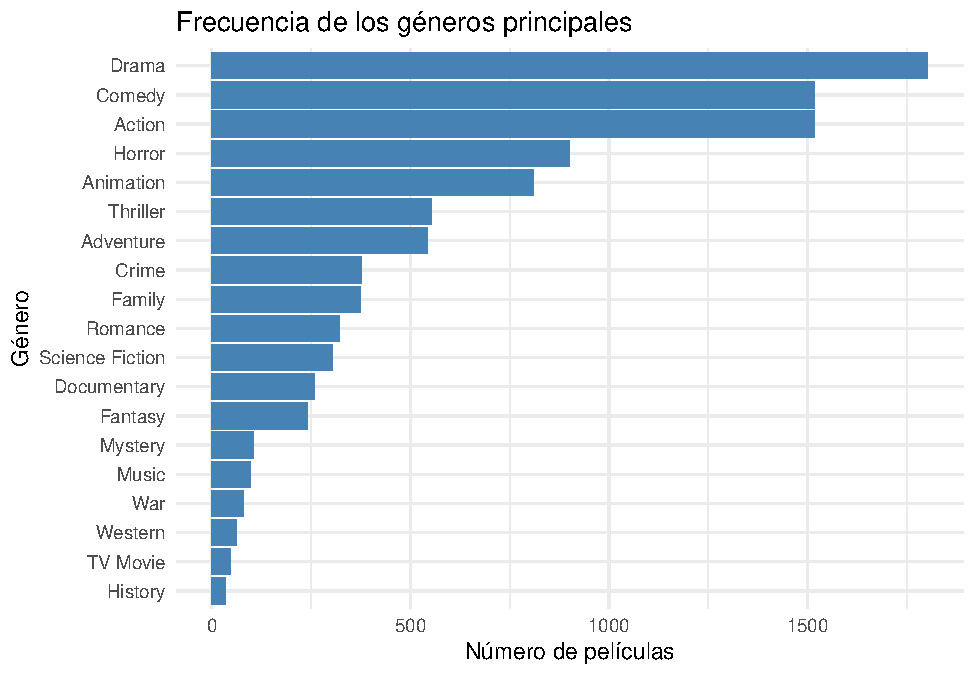
\includegraphics{Preguntas_Exploratorias2_files/figure-latex/unnamed-chunk-8-1.pdf}
\includegraphics{Preguntas_Exploratorias2_files/figure-latex/unnamed-chunk-8-2.pdf}
\includegraphics{Preguntas_Exploratorias2_files/figure-latex/unnamed-chunk-8-3.pdf}

Como se puede observar, si hay una tendencia y relación clara entre el
budget y el revenue. Aunque un budget alto no represente siempre un
pexito, es claro que mientras mayor presupuesto tenga la película, más
oportunidad de generar ganancias tiene. A medida que incremente el
presupuesto también lo hacen las ganacias.

\subsubsection{13 ¿En qué meses se han visto los lanzamientos con
mejores ingresos? ¿cuantas películas, en promedio, se han lanzado por
mes?}\label{en-quuxe9-meses-se-han-visto-los-lanzamientos-con-mejores-ingresos-cuantas-peluxedculas-en-promedio-se-han-lanzado-por-mes}

\begin{verbatim}
##      mes_texto    revenue                                         title
## 3211  December 2847246203                                        Avatar
## 5953     April 2797800564                             Avengers: Endgame
## 308   November 2187463944                                       Titanic
## 4948  December 2068223624                  Star Wars: The Force Awakens
## 5954     April 2046239637                        Avengers: Infinity War
## 4915      June 1671713208                                Jurassic World
## 7135      July 1667635327                                 The Lion King
## 9050  December 1631853496                       Spider-Man: No Way Home
## 3398     April 1518815515                                  The Avengers
## 5088     April 1515047671                                     Furious 7
## 6181  November 1450026933                                     Frozen II
## 4711     April 1405403694                       Avengers: Age of Ultron
## 5799  February 1346739107                                 Black Panther
## 2510      July 1341511219  Harry Potter and the Deathly Hallows: Part 2
## 5149  December 1332698830                      Star Wars: The Last Jedi
## 6429      June 1303459585                Jurassic World: Fallen Kingdom
## 4766  November 1274219009                                        Frozen
## 6109     March 1263521126                          Beauty and the Beast
## 5626      June 1242805359                                 Incredibles 2
## 6272     April 1238764765                       The Fate of the Furious
## 4339     April 1214811252                                    Iron Man 3
## 5302      June 1156730962                                       Minions
## 5702     April 1153296293                    Captain America: Civil War
## 5940      July 1148461807                                       Aquaman
## 7240      June 1131927996                     Spider-Man: Far From Home
## 5955     March 1128276090                                Captain Marvel
## 3772      June 1123794079                Transformers: Dark of the Moon
## 69    December 1118888979 The Lord of the Rings: The Return of the King
## 3736   October 1108561013                                       Skyfall
## 4666      June 1100000000               Transformers: Age of Extinction
\end{verbatim}

El promedio de peliculas por mes en general es \textbf{833.3333333}. A
continuación se meustra como se distribuyen las peliculas en los meses
del anio.

\begin{verbatim}
## # A tibble: 12 x 2
##    mes_texto cantidad_peliculas
##    <chr>                  <int>
##  1 April                    696
##  2 August                   913
##  3 December                 935
##  4 February                 706
##  5 January                  652
##  6 July                     812
##  7 June                     819
##  8 March                    815
##  9 May                      698
## 10 November                 807
## 11 October                 1068
## 12 September               1079
\end{verbatim}

\subsubsection{15 ¿La popularidad del elenco está directamente
correlacionada con el éxito de
taquilla?}\label{la-popularidad-del-elenco-estuxe1-directamente-correlacionada-con-el-uxe9xito-de-taquilla}

\begin{verbatim}
## `geom_smooth()` using formula = 'y ~ x'
\end{verbatim}

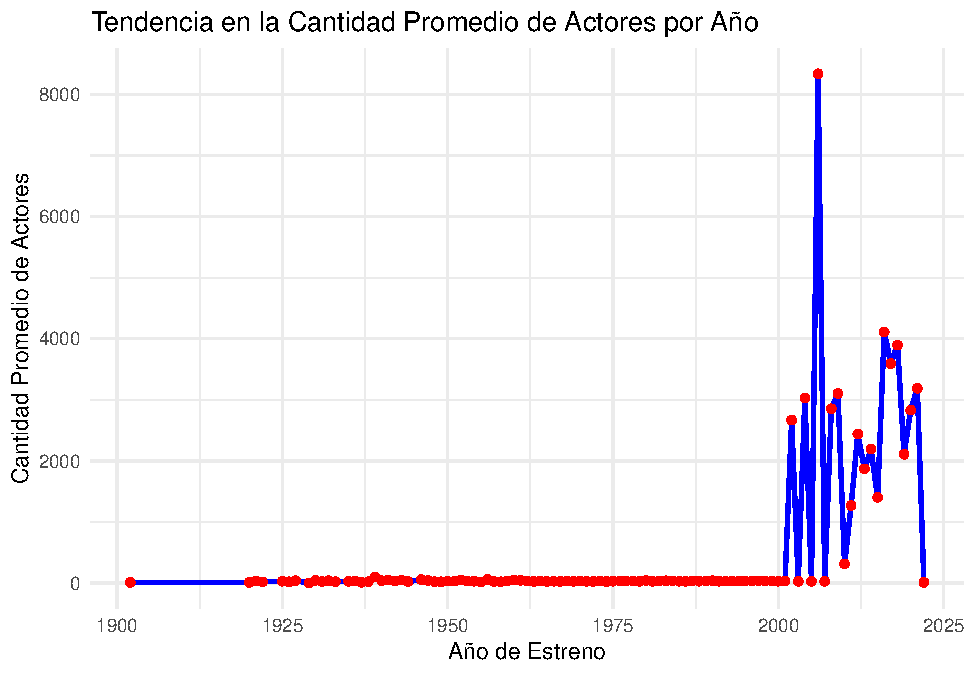
\includegraphics{Preguntas_Exploratorias2_files/figure-latex/unnamed-chunk-12-1.pdf}

Al final se tiene un coeficiente de \textbf{0.5492487}. Lo cual indica
que hay una correlacion entre la popularidad del elenco y las ganancias
y exito en taquilla. Aunque no se tan alto si existen una relacion entre
ambas variables.

\subsubsection{Extras}\label{extras}

\subsubsection{¿Cuales son los 10 lenguajes originales mas comunes entre
todas las
peliculas?}\label{cuales-son-los-10-lenguajes-originales-mas-comunes-entre-todas-las-peliculas}

\begin{verbatim}
## # A tibble: 10 x 2
##    originalLanguage cantidad_len
##    <chr>                   <int>
##  1 en                       7772
##  2 ja                        644
##  3 es                        425
##  4 fr                        271
##  5 ko                        167
##  6 zh                        119
##  7 it                        100
##  8 de                         84
##  9 cn                         80
## 10 ru                         67
\end{verbatim}

\includegraphics{Preguntas_Exploratorias2_files/figure-latex/unnamed-chunk-13-1.pdf}

\subsubsection{¿Hay alguna correlación entre el largo de la pelicula y
su popularidad? Son populares las peliculas
largas?}\label{hay-alguna-correlaciuxf3n-entre-el-largo-de-la-pelicula-y-su-popularidad-son-populares-las-peliculas-largas}

\begin{verbatim}
##      runtime popularity
## 9348     750     12.190
## 5359     400     25.716
## 3886     333     11.224
## 963      317     11.607
## 1264     248     45.072
## 7066     247     23.168
## 1949     242     12.449
## 9687     242    628.372
## 3741     240     16.700
## 5593     240     24.845
## 6160     240     15.204
## 2949     237     12.369
## 415      233     32.151
## 9220     231     12.326
## 177      229     45.994
## 517      227     33.961
## 365      222     47.378
## 1169     220     66.514
## 4278     213     30.499
## 9769     213     14.382
\end{verbatim}

\begin{verbatim}
## `geom_smooth()` using formula = 'y ~ x'
\end{verbatim}

\includegraphics{Preguntas_Exploratorias2_files/figure-latex/unnamed-chunk-14-1.pdf}

\begin{verbatim}
## [1] "El coeficiente de correlacion es: 0.03"
\end{verbatim}

Al final se puede observar que realmente no hay una alta correlación
entre la duración de la película y su popularidad. Si una película es
larga o corta no debería de influir en la popularidad de la película.

El coeficiente de correlación entre la duracion de la pelicula y su
popularidaa es \textbf{0.03}

\subsubsection{¿Las peliculas con meyor budget tienen mejores notas
promedio?}\label{las-peliculas-con-meyor-budget-tienen-mejores-notas-promedio}

\begin{verbatim}
##      voteAvg    budget
## 717      6.5 380000000
## 4711     7.3 365000000
## 5953     8.3 356000000
## 164      7.2 300000000
## 4954     6.2 300000000
## 5954     8.3 300000000
## 608      5.7 270000000
## 3792     7.6 260000000
## 7135     7.1 260000000
## 281      6.3 258000000
## 412      7.7 250000000
## 2509     7.8 250000000
## 4035     7.8 250000000
## 4039     7.3 250000000
## 4052     6.2 250000000
## 4179     7.6 250000000
## 4856     7.3 250000000
## 4881     7.5 250000000
## 5150     6.5 250000000
## 5280     5.9 250000000
\end{verbatim}

\begin{verbatim}
## `geom_smooth()` using formula = 'y ~ x'
\end{verbatim}

\includegraphics{Preguntas_Exploratorias2_files/figure-latex/unnamed-chunk-15-1.pdf}

Se obtuvo un coeficiente de \textbf{0.04}. Lo cual indica que el
presupuesto de una pelicula no influye para nada en la nota promedio de
la pelicula. un buen budget no implica buenas criticas.

\end{document}
